%% abtex2-modelo-relatorio-tecnico.tex, v-1.9.5 laurocesar
%% Copyright 2012-2015 by abnTeX2 group at http://www.abntex.net.br/ 
%%
%% This work may be distributed and/or modified under the
%% conditions of the LaTeX Project Public License, either version 1.3
%% of this license or (at your option) any later version.
%% The latest version of this license is in
%%   http://www.latex-project.org/lppl.txt
%% and version 1.3 or later is part of all distributions of LaTeX
%% version 2005/12/01 or later.
%%
%% This work has the LPPL maintenance status `maintained'.
%% 
%% The Current Maintainer of this work is the abnTeX2 team, led
%% by Lauro César Araujo. Further information are available on 
%% http://www.abntex.net.br/
%%
%% This work consists of the files abntex2-modelo-relatorio-tecnico.tex,
%% abntex2-modelo-include-comandos and abntex2-modelo-references.bib
%%

% ------------------------------------------------------------------------
% ------------------------------------------------------------------------
% abnTeX2: Modelo de Relatório Técnico/Acadêmico em conformidade com 
% ABNT NBR 10719:2011 Informação e documentação - Relatório técnico e/ou
% científico - Apresentação
% ------------------------------------------------------------------------ 
% ------------------------------------------------------------------------

\documentclass[
	% -- opções da classe memoir --
	12pt,				% tamanho da fonte
	openright,			% capítulos começam em pág ímpar (insere página vazia caso preciso)
	oneside,			% para impressão em verso e anverso. Oposto a oneside
	a4paper,			% tamanho do papel. 
	% -- opções da classe abntex2 --
	%chapter=TITLE,		% títulos de capítulos convertidos em letras maiúsculas
	%section=TITLE,		% títulos de seções convertidos em letras maiúsculas
	%subsection=TITLE,	% títulos de subseções convertidos em letras maiúsculas
	%subsubsection=TITLE,% títulos de subsubseções convertidos em letras maiúsculas
	% -- opções do pacote babel --
	english,			% idioma adicional para hifenização
	french,				% idioma adicional para hifenização
	spanish,			% idioma adicional para hifenização
	brazil,				% o último idioma é o principal do documento
	]{abntex2}


% ---
% PACOTES
% ---

% ---
% Pacotes fundamentais 
% ---
\usepackage{lmodern}			% Usa a fonte Latin Modern
\usepackage[T1]{fontenc}		% Selecao de codigos de fonte.
\usepackage[utf8]{inputenc}		% Codificacao do documento (conversão automática dos acentos)
\usepackage{indentfirst}		% Indenta o primeiro parágrafo de cada seção.
\usepackage{color}				% Controle das cores
\usepackage{graphicx}			% Inclusão de gráficos
\usepackage{microtype} 			% para melhorias de justificação
% ---

% ---
% Pacotes adicionais, usados no anexo do modelo de folha de identificação
% ---
\usepackage{multicol}
\usepackage{multirow}
\usepackage{epstopdf}
% ---
	
% ---
% Pacotes adicionais, usados apenas no âmbito do Modelo Canônico do abnteX2
% ---
\usepackage{lipsum}				% para geração de dummy text
% ---

% ---
% Pacotes de citações
% ---
\usepackage[brazilian,hyperpageref]{backref}	 % Paginas com as citações na bibl
\usepackage[alf]{abntex2cite}	% Citações padrão ABNT

% ---
% Informações de dados para CAPA e FOLHA DE ROSTO
% ---
\titulo{Controle de Motor BLDC \\ Ponto de Verificação 2}
\autor{Afonso Menegola \& Braian Zanini}
\local{Porto Alegre}
\data{2015}
\instituicao{%
  Universidade Federal do Rio Grande do Sul -- UFRGS
  \par
  Departamento de Engenharia Elétrica
}
\tipotrabalho{Relatório técnico}
% O preambulo deve conter o tipo do trabalho, o objetivo, 
% o nome da instituição e a área de concentração 
\preambulo{Relatório técnico referente ao Ponto de Verificação 2 da disciplina ENG04073 - Sistemas de Controle Eletroeletrônicos do curso de graduação em Engenharia Elétrica da Universidade Federal do Rio Grande do Sul}
% ---

% ---
% Configurações de aparência do PDF final

% alterando o aspecto da cor azul
\definecolor{blue}{RGB}{0,0,0}

% informações do PDF
\makeatletter
\hypersetup{
     	%pagebackref=true,
		pdftitle={\@title}, 
		pdfauthor={\@author},
    	pdfsubject={\imprimirpreambulo},
	    pdfcreator={LaTeX with abnTeX2},
		pdfkeywords={abnt}{latex}{abntex}{abntex2}{relatório técnico}, 
		colorlinks=true,       		% false: boxed links; true: colored links
    	linkcolor=blue,          	% color of internal links
    	citecolor=blue,        		% color of links to bibliography
    	filecolor=magenta,      		% color of file links
		urlcolor=blue,
		bookmarksdepth=4
}
\makeatother
% --- 

% --- 
% Espaçamentos entre linhas e parágrafos 
% --- 

% O tamanho do parágrafo é dado por:
\setlength{\parindent}{1.3cm}

% Controle do espaçamento entre um parágrafo e outro:
\setlength{\parskip}{0.2cm}  % tente também \onelineskip

% ---
% compila o indice
% ---
\makeindex
% ---

% ----
% Início do documento
% ----
\begin{document}

% Seleciona o idioma do documento (conforme pacotes do babel)
%\selectlanguage{english}
\selectlanguage{brazil}

% Retira espaço extra obsoleto entre as frases.
\frenchspacing 

% ----------------------------------------------------------
% ELEMENTOS PRÉ-TEXTUAIS
% ----------------------------------------------------------
% \pretextual

% ---
% Capa
% ---
\imprimircapa
% ---

% ---
% Folha de rosto
% (o * indica que haverá a ficha bibliográfica)
% ---
\imprimirfolhaderosto*
% ---


% ---
% RESUMO
% ---

% resumo na língua vernácula (obrigatório)
\setlength{\absparsep}{18pt} % ajusta o espaçamento dos parágrafos do resumo
\begin{resumo}
 Segundo a NBR, o resumo deve ressaltar o
 objetivo, o método, os resultados e as conclusões do documento. A ordem e a extensão
 destes itens dependem do tipo de resumo (informativo ou indicativo) e do
 tratamento que cada item recebe no documento original. O resumo deve ser
 precedido da referência do documento, com exceção do resumo inserido no
 próprio documento. (\ldots) As palavras-chave devem figurar logo abaixo do
 resumo, antecedidas da expressão Palavras-chave:, separadas entre si por
 ponto e finalizadas também por ponto.

 \noindent
 \textbf{Palavras-chaves}: latex. abntex. editoração de texto.
\end{resumo}
% ---

% ---
% inserir lista de ilustrações
% ---
\pdfbookmark[0]{\listfigurename}{lof}
\listoffigures*
\cleardoublepage
% ---

% ---
% inserir lista de tabelas
% ---
\pdfbookmark[0]{\listtablename}{lot}
\listoftables*
\cleardoublepage
% ---

% ---
% inserir lista de abreviaturas e siglas
% ---
\begin{siglas}
  \item[CC] Corrente Contínua
  \item[CA] Corrente Alternada
	\item[BLDC] \textit{Brushless Direct Current}
\end{siglas}
% ---

% ---
% inserir lista de símbolos
% ---
\begin{simbolos}
  \item[$ e $] Força Eletromotriz Inversa
  \item[$ \omega $] Velocidade Angular
  \item[$ k_f $] Constante de Fricção
  \item[$ k_e $] Constante de Tensão
  \item[$ k_t $] Constante de Torque
	\item[$ \tau_m $] Constante de Tempo Mecânica
	\item[$ \tau_e $] Constante de Tempo Elétrica
\end{simbolos}
% ---

% ---
% inserir o sumario
% ---
\pdfbookmark[0]{\contentsname}{toc}
\tableofcontents*
\cleardoublepage
% ---


% ----------------------------------------------------------
% ELEMENTOS TEXTUAIS
% ----------------------------------------------------------
\textual

% ----------------------------------------------------------
% Introdução (exemplo de capítulo sem numeração, mas presente no Sumário)
% ----------------------------------------------------------
\chapter*[Introdução]{Introdução}
\addcontentsline{toc}{chapter}{Introdução}

Motores CC têm sido usados na indústria por muitos anos. Eles possuem uma alta eficiência e possuem alto torque inicial que ajuda a prevenir problemas como o aumento da carga de uma forma abrupta \cite{dcPrinciples}. Entretanto, motores CC possuem algumas deficiências, tais como desgaste físico através do uso de escovas para comutação, faiscamento, ruído acústico, entre outros. Tais problemas resultaram no desenvolvimento de novos motores síncronos sem a utilização de escovas. Os motores de corrente contínua sem escovas (do Inglês \textit{Brushless Direct Current}) ou motores BLDC, eliminam os defeitos argumentados e possuem diversas aplicações, como por exemplo aeronáutica, medicina, automação residencial e industrial, etc.

Motores BLDC são motores síncronos alimentados por uma fonte CC, e por esse motivo que são chamados de motores de corrente contínua, já que a comutação é realizada através de um inversor de potência que produz um sinal elétrico CA ao motor, onde nesse contexto não é uma onda sinusoidal, mas uma corrente bidirecional sem restrição na forma de onda.

Algumas vantagens do motor BLDC em relação ao motor CC são apresentados \cite{brushFundamentals}:

\begin{enumerate}
	\item Melhores características de velocidade versus torque
	\item Alta resposta dinâmica
	\item Baixo nível de ruído sonoro
	\item Maiores velocidades
	\item Baixa manutenção
	\item Alto torque comparado ao tamanho da sua estrutura
\end{enumerate}

O motor BLDC pode ser construído com diferentes fases, na qual o mais comum é o trifásico. Apesar disso, suas características elétricas e físicas se assemelham muito ao motor CC, e é através dessa semelhança que o presente projeto irá buscar a modelagem e identificação de um motor BLDC.

O relatório se apresenta na seguinte sequência: no capítulo 1 a apresentação e modelagem de um motor CC serão realizadas. No capítulo 2, a modelagem do motor BLDC é realizada buscando a semelhança dos dois motores. O capítulo 3 explica os passos dos ensaios realizados com o motor \textit{E-flite Park} 300 para a obtenção de suas características elétricas e mecânicas. Os passos para identificação são versados no capítulo 4. Os resultados da modelagem e identificação do motor citado são apresentados no capítulo 5 e, finalmente, são realizadas as conclusões sobre o progresso realizado.
% ----------------------------------------------------------
% Capitulo com exemplos de comandos inseridos de arquivo externo 
% ----------------------------------------------------------

\chapter{Modelagem de Motores CC}

\section{Motores CC}

Uma máquina de corrente contínua possui quatro partes principais: O rotor (também chamado de armadura), o comutador o estator e as escovas. Uma representação de tais partes podem ser visualizadas na \autoref{figMotorDC}.

O rotor é a parte girante montada sobre o eixo da máquina, constituído de um material ferromagnético envolto em um enrolamento chamado de enrolamento de armadura. É o circuito responsável por transportar a energia proveniente da fonte de energia.

O comutador é responsável por realizar a inversão adequada do sentido das correntes que circulam no enrolamento de armadura, constituído de um anel de material condutor, segmentado por um material isolante de forma a fechar o circuito entre cada uma das bobinas do enrolamento de armadura e as escovas no momento adequado.

O estator é a parte estática da máquina, montada em volta do rotor, de forma que o mesmo possa girar internamente. No caso do nosso projeto, o estator possui ímãs que tem a função apenas de produzir um campo magnético fixo para interagir com o campo da armadura.

As escovas são peças de grafite responsáveis por conduzir a energia para o circuito do rotor.

\begin{figure}[htb]
	\caption{\label{figMotorDC}Partes Constituintes de um Motor de Corrente Contínua}
	\begin{center}
	  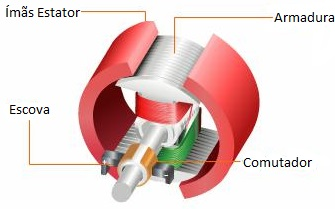
\includegraphics{figuras/dcMotorParts.jpeg}
	\end{center}
	\legend{Fonte: http://images.tutorvista.com/content/magnetic-effects-electric-current}
\end{figure}

\section{Modelo do Motor CC}

Um arranjo típico eletromecânico de um motor CC está representado na \autoref{figEletromechSys}. Os componentes básicos do circuito representado são a resistência de armadura \textit{R}, a indutância \textit{L} e a força eletromotriz inversa \textit{e}.

\begin{figure}[htb]
	\caption{\label{figEletromechSys}Arranjo típico de um sistema eletromecânico do motor CC}
	\begin{center}
	  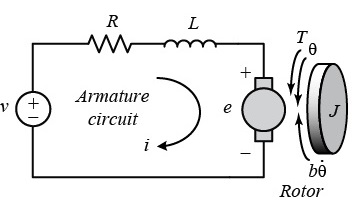
\includegraphics{figuras/dcEletroMech.jpg}
	\end{center}
	\legend{Fonte: http://ctms.engin.umich.edu/CTMS/Content/MotorSpeed/}
\end{figure}

Aplicando a Lei das Tensões de Kirchhoff, a \autoref{kvl} é obtida.

\begin{equation}
\label{kvl}
  V = Ri + L\frac{\partial i}{\partial t} + e
\end{equation}

Onde $V$ é a tensão de alimentação e $i$ é a corrente de armadura.

Utilizando a segunda Lei de Newton as grandezas mecânicas são relacionadas de acordo com a \autoref{newton} e, substituindo as respectivas grandezas, a equação que descreve o torque é representado pela \autoref{torque}.

\begin{equation}
\label{newton}
  J\frac{\partial \omega}{\partial t} = \sum{T_i}
\end{equation}
\begin{equation}
\label{torque}
  T_e = k_f\omega + J\frac{\partial \omega}{\partial t} +T_L
\end{equation}

Onde,\\
$T_e$ = torque elétrico\\
$k_f$ = constante de fricção\\
$J$ = inércia do rotor\\
$\omega$ = velocidade angular\\
$T_L$ = carga externa

A força eletromotriz inversa e o torque elétrico também podem ser escritos de acordo com a \autoref{backemf} e a \autoref{teletr}, respectivamente.

\begin{equation}
\label{backemf}
  e = k_e\omega
\end{equation}
\begin{equation}
\label{teletr}
  T_e = k_t\omega
\end{equation}

Onde,\\
$k_e$ = constante de tensão\\
$k_t$ = constante de torque\\

Reescrevendo então a \autoref{kvl} e a \autoref{newton} utilizando as equações anteriores, a \autoref{primeiradiferencial} e a \autoref{segundadiferencial} são obtidas.

\begin{equation}
\label{primeiradiferencial}
  \frac{\partial i}{\partial t} = -i\frac{R}{L} - \frac{k_e}{L}\omega + \frac{1}{L}V
\end{equation}
\begin{equation}
\label{segundadiferencial}
  \frac{\partial \omega}{\partial t} = i \frac{k_t}{J} - \frac{k_f}{J}\omega + \frac{1}{J}T_L
\end{equation}

Aplica-se Laplace na \autoref{primeiradiferencial} e na \autoref{segundadiferencial} para o caso de nenhuma carga externa aplicada, obtém-se a \autoref{primlaplace} e a \autoref{seglaplace}

\begin{equation}
\label{primlaplace}
  si = -i\frac{R}{L} - \frac{k_e}{L}\omega + \frac{1}{L}V
\end{equation}
\begin{equation}
\label{seglaplace}
  s\omega = i\frac{k_t}{J} - \frac{k_f}{J}\omega
\end{equation}

Isolando e substituindo a corrente $i$ da \autoref{seglaplace} na \autoref{primlaplace} e isolando $V$, obtém-se a \autoref{visolado}

\begin{equation}
\label{visolado}
  V = \left\{\frac{s^2JL + sk_fL + sRJ + k_fR + k_ek_t}{k_t}\right\}\omega
\end{equation}

Finalmente, a \autoref{functrans} é obtida através de alguns passos algébricos.

\begin{equation}
\label{functrans}
  G(S) = \frac{\omega}{V} = \frac{k_t}{s^2JL + (RJ + k_fL)s + k_fR + k_ek_t}
\end{equation}

Supondo o coeficiente de fricção muito pequeno, a \autoref{functrans} pode ser simplificada e rearranjada na \autoref{functranssimpl}.

\begin{equation}
\label{functranssimpl}
  G(S) = \frac{\frac{1}{k_e}}{\frac{RJ}{k_ek_t}.\frac{L}{R}.s^2 + \frac{RJ}{k_ek_t}.s + 1}
\end{equation}

Da \autoref{functranssimpl} duas constantes são obtidas, a constante de tempo mecânica e a constante de tempo elétrica.

\begin{equation}
\label{mecConst}
  \tau_m = \frac{RJ}{k_ek_t}
\end{equation}
\begin{equation}
\label{eleConst}
  \tau_e = \frac{L}{R}
\end{equation}

Substituindo tais constantes na \autoref{functranssimpl} a \autoref{functranstime} é obtida.

\begin{equation}
\label{functranstime}
  G(S) = \frac{\frac{1}{k_e}}{\tau_m.\tau_e.s^2 + \tau_m.s + 1}
\end{equation}

\chapter{Modelagem de Motores BLDC}

\section{Motores BLDC}

Uma das maiores diferenças entre o motor CC e o BLDC é a adição de mais fases. No caso do presente projeto, o motor BLDC utilizado possui três fases. Diferentemente do motor CC, a comutação é realizada através de controle eletrônico. Os enrolamentos do estator, nesse caso, são energizados em sequência para o motor girar. Uma representação do motor BLDC pode ser encontrado na \autoref{figbldc}.

\begin{figure}[htb]
	\caption{\label{figbldc}Motor BLDC}
	\begin{center}
	  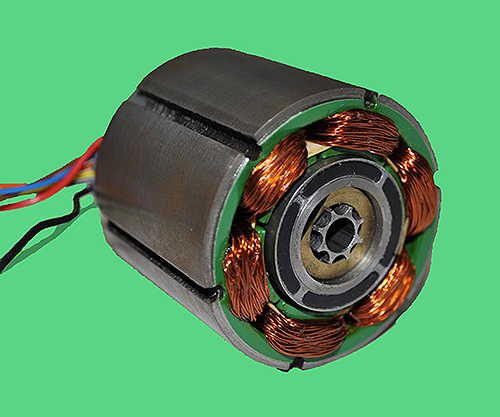
\includegraphics[scale=0.4]{figuras/figbldc.jpg}
	\end{center}
	\legend{Fonte: http://www.designworldonline.com/}
\end{figure}

Tipicamente, o modelo matemático de um motor BLDC não difere muito de um motor CC convencional. As fases extras é a modificação principal que afetam os valores das constantes do sistema eletromecânico equivalente.

\begin{figure}[htb]
	\caption{\label{figbldcsys}Arranjo típico de um sistema elétrico do motor BLDC}
	\begin{center}
	  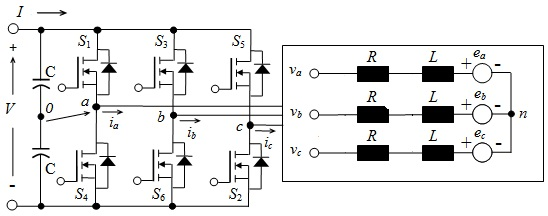
\includegraphics{figuras/figbldcsys.jpg}
	\end{center}
	\legend{Fonte: http://www.intechopen.com/source/}
\end{figure}

Utilizando a simetria do arranjo ilustrado na \autoref{figbldcsys}, a constante mecânica e elétrica podem ser expressas pela \autoref{taum} e \autoref{taue}.

\begin{equation}
\label{taum}
  \tau_m = \frac{3RJ}{k_ek_t}
\end{equation}
\begin{equation}
\label{taue}
  \tau_e = \frac{L}{3R}
\end{equation}

A função de transferência, portanto, permanece a mesma da \autoref{functranstime}. Para conseguirmos validar a modelagem e realizar a identificação, é necessário portanto somente descobrir as constantes de tempo. Geralmente, os fabricantes fornecem essas informações para motores BLDC de uso comercial. O motor utilizado para o desenvolvimento deste projeto, entretanto, é o motor \textit{E-flite Park} 300, um motor utilizado em aeromodelismo, e, portanto, o fabricante não fornece as informações necessárias para a determinação de tais constantes.

De forma que se consiga prosseguir a análise matemática da modelagem do motor BLDC utilizado, se faz necessária a sua caracterização elétrica e mecânica. O motor BLDC utilizado na identificação do sistema é um motor típico em aplicações de aeromodelismo, e, portanto, a fabricante não fornece os parâmetros necessários para a modelagem. O procedimento experimental para a caracterização do motor será discutido na próxima seção, entretanto, tal procedimento não foi realizado. A propagação do erro associado às medições que seriam feitas através de instrumentos com baixa precisão disponíveis iria causar uma grande diferença entre a resposta ao salto calculado pela modelagem e pela identificação, não podendo, portanto, ser realizada uma comparação entre os dois resultados.

\section{Caracterização Elétrica e Mecânica}

Para obter as constantes de tempo necessárias para a correta modelagem do motor utilizado, é necessário obter as constantes relacionadas à \autoref{taum} e \autoref{taue} para cada fase do motor.

Portanto, devemos obter:

\begin{itemize}
	\item Resistência
	\item Indutância
	\item Constante de tensão
	\item Constante de torque
	\item Inércia do rotor
\end{itemize}

\subsection{Resistência}

Como a resistência de fase de um motor BLDC é considerada igual entre suas fases, é realizada a medição de resistência entre duas fases e, após, a divisão desse valor por dois.

\subsection{Indutância}

Para a medição da indutância de fase do motor BLDC utiliza-se um gerador de função para produzir de um sinal CA de baixa amplitude, o qual deve ser aplicado a um par de fases. A tensão rms entre as fases do motor, dividida  pela corrente rms resulta na impedância $X$ de linha. A indutância é então calculada através da \autoref{indutancia}.

\begin{equation}
\label{indutancia}
  L = \frac{\sqrt{X^2 - R^2}}{4\pi f}
\end{equation}

\subsection{Constante de tensão}

Deve-se excitar o motor até uma velocidade $v$ em $rad/s$. De posse do valor dessa velocidade,  pode-se utilizar um multímetro para a obtenção da tensão rms entre duas fases do motor. A constante de tensão de fase é então calculada através da \autoref{cteTensao}.

\begin{equation}
\label{cteTensao}
  k_e = \frac{V_{rms}}{\sqrt{3} v}
\end{equation}

\subsection{Constante de torque}

Pode-se demonstrar \cite{referenceBook} que a constante de torque para um motor BLDC obedece a \autoref{cteTorque}.

\begin{equation}
\label{cteTorque}
  k_t = 16,53 \times k_e
\end{equation}

\subsection{Momento de Inércia do Rotor}

Como o rotor do motor utilizado aproxima-se de um tubo cilíndrico (\autoref{figCilindro}), o momento de inércia pode ser calculado através da \autoref{eq:inercia} sabendo a massa e os raios interno e externo do rotor.

\begin{equation}
\label{eq:inercia}
  I = \frac{1}{2}m\left(r_1^2 + r_1^2\right)
\end{equation}

\begin{figure}[htb]
	\caption{\label{figCilindro}Tubo cilíndrico}
	\begin{center}
	  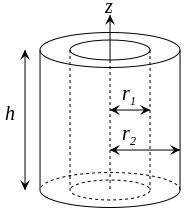
\includegraphics[scale=0.5]{figuras/figcilindro.png}
	\end{center}
	\legend{Fonte: https://en.wikipedia.org/wiki/List\_of\_moments\_of\_inertia}
\end{figure}

\chapter{Identificação}
Escrever

\section{Exemplo de seção}

As paradas

\chapter{Resultados}
Escrever

\section{Exemplo de seção}

As paradas

% ---
% Finaliza a parte no bookmark do PDF
% para que se inicie o bookmark na raiz
% e adiciona espaço de parte no Sumário
% ---
\phantompart

% ---
% Conclusão
% ---
\chapter{Conclusão}
% ---

Escrever Conclusão

% ----------------------------------------------------------
% ELEMENTOS PÓS-TEXTUAIS
% ----------------------------------------------------------
\postextual

% ----------------------------------------------------------
% Referências bibliográficas
% ----------------------------------------------------------
\bibliography{referencias}

% ----------------------------------------------------------
% Glossário
% ----------------------------------------------------------
%
% Consulte o manual da classe abntex2 para orientações sobre o glossário.
%
%\glossary

% ----------------------------------------------------------
% Apêndices
% ----------------------------------------------------------

% ---
% Inicia os apêndices
% ---
\begin{apendicesenv}

% Imprime uma página indicando o início dos apêndices
\partapendices

% ----------------------------------------------------------
\chapter{Exemplo de Apêndice}
% ----------------------------------------------------------

Escrever caso necessário.

\end{apendicesenv}
% ---


% ----------------------------------------------------------
% Anexos
% ----------------------------------------------------------

% ---
% Inicia os anexos
% ---
\begin{anexosenv}

% Imprime uma página indicando o início dos anexos
\partanexos

% ---
\chapter{Exemplo de capítulo em anexo}
% ---
Escrever caso necessário

\end{anexosenv}



\end{document}
